\chapter{Specific requirements}

% TODO: definition in separate datei packen (und evtl. verbessern)
\newcommand{\funcRequirement}[6]{
\begin{center}
\begin{tabular}{|l|p{12cm}|}
\hline
Req. ID 		& #1 \\ \hline
Name 				& #2 \\ \hline
Description & #3 \\ \hline
Priority 		& #4 \\ \hline
Comment 		& #5 \\ \hline
\end{tabular}
\end{center}
}

\newcommand{\nonFuncRequirement}[6]{
\begin{center}
\begin{tabular}{|l|p{12cm}|}
\hline
Req. ID 		 & #1 \\ \hline
Name 				 & #2 \\ \hline
Beschreibung & #3 \\ \hline
Typ 				 & #4 \\ \hline
Priorität 	 & #5 \\ \hline
Anmerkung    & #6\\ \hline
\end{tabular}
\end{center}
}


	\section{Functional requirements}

	\subsection{Use Cases}
	
	\begin{figure}[!h]
		\centering
			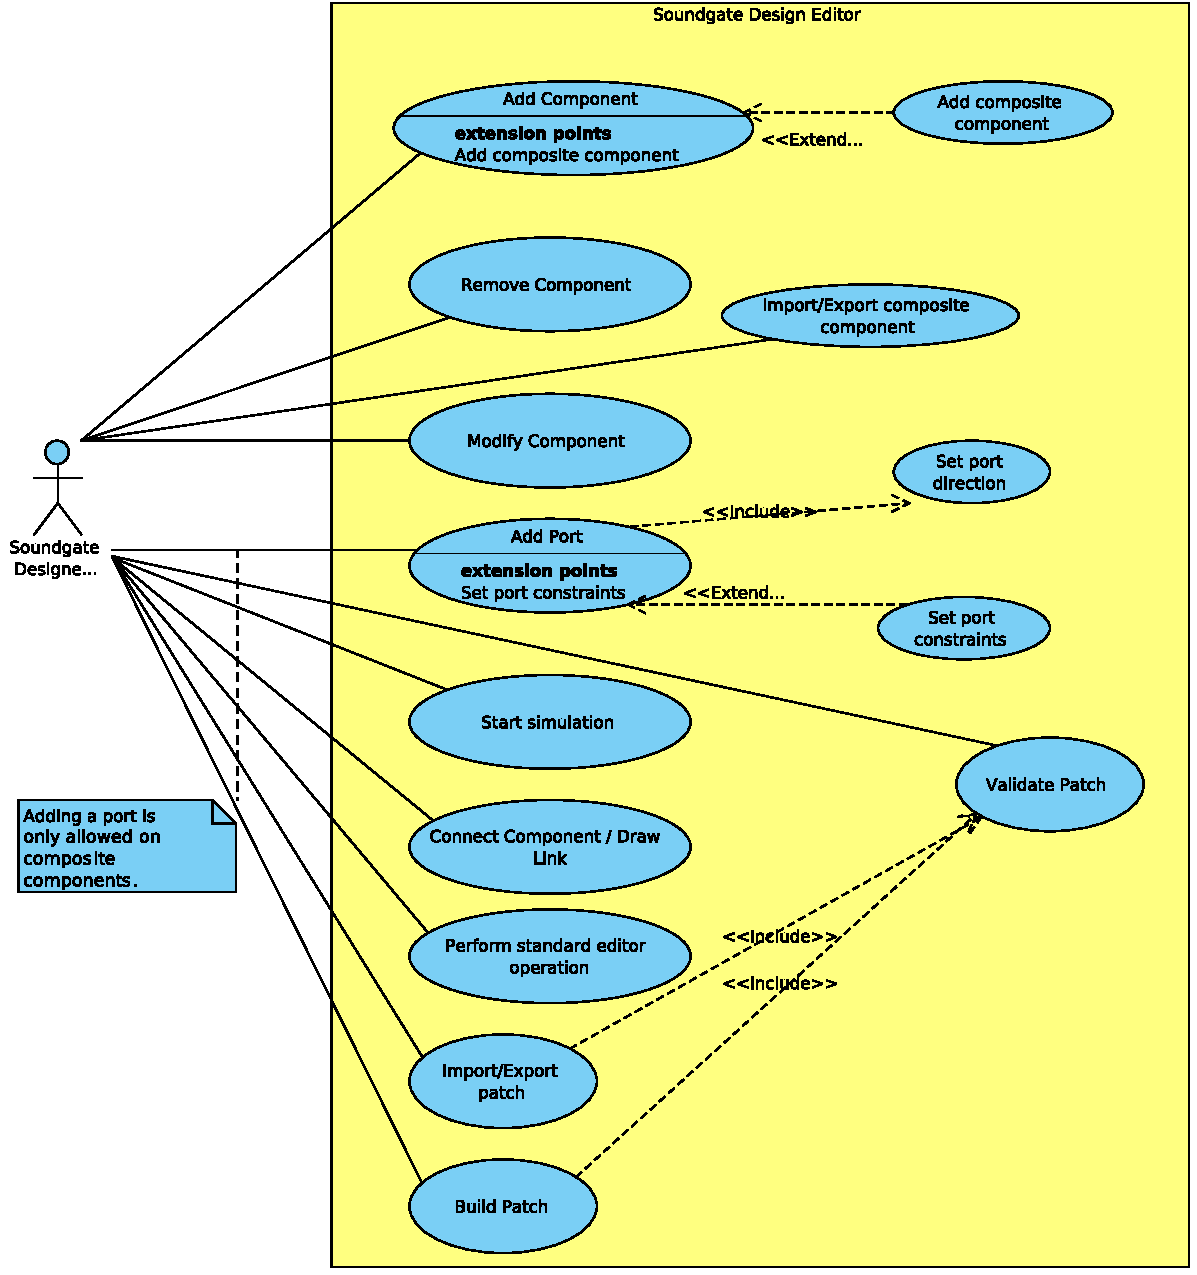
\includegraphics[width=0.93\textwidth]{images/Soundgate_Designer.pdf}
		\caption{Use case diagram of the soundgate designer (editor)}
		\label{fig:Soundgate_Designer}
	\end{figure}
	
	\begin{figure}[!h]
		\centering
			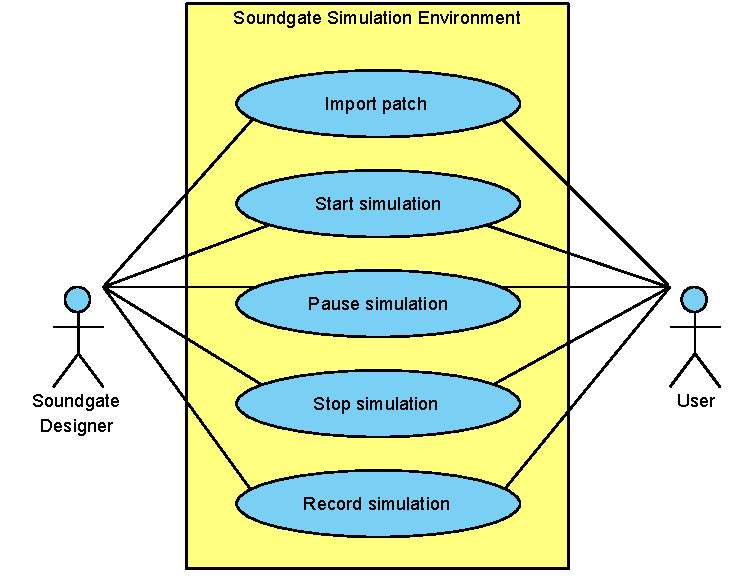
\includegraphics[width=0.90\textwidth]{images/Soundgate_Simulator.pdf}
		\caption{Use case diagram of the soundgate simulation environment}
		\label{fig:Soundgate_Simulator}
	\end{figure}
	
	\begin{figure}[!h]
		\centering
			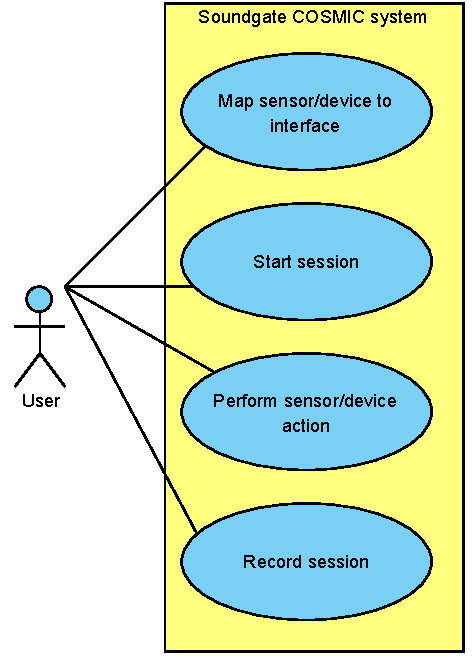
\includegraphics[width=0.90\textwidth]{images/User_View.pdf}
		\caption{Use case diagram of the soundgate user interface}
		\label{fig:Soundgate_UserInterface}
	\end{figure}
	\FloatBarrier
	\funcRequirement{1.1}
	{Add component to a patch}
	{The soundgate designer (SD) must be able to add components to a patch.}
	{high}
	{--}
	
  \funcRequirement{1.2}
	{Remove component from a path}
	{The SD must be able to remove components from a patch.}
	{high}
	{--}
	
  \funcRequirement{1.3}
	{Modify attributes of a component}
	{The SD should be able to modify static parameters of a component.}
	{mid}
	{The values of static parameters, like the channel of an audio output interface, must not be changed outside of the designing time.}
	
	\funcRequirement{1.4}
	{Add composite components}
	{The SD user must be able to create composite components.}
	{The SD must be able to create composite components.}
	{mid}
	{The priority is classified as medium, because a correct patch could be created without composite components. }
	
	\funcRequirement{1.5}
	{Add port to a composite component}
	{The SD must be able to add a port to a composite component.}
	{mid}
	{Only composite components can have user defined ports. Ports of atomic components are fixed, such they cannot be added, removed or modified.}
	
	\funcRequirement{1.5.1}
	{Set port direction}
	{The SD must be able to set the direction of a port.}
	{mid}
	{A port is either incoming or outgoing.}
	
	\funcRequirement{1.5.2}
	{Set port constraints}
	{The SD should be able to add constraints to a port.}
	{mid}
	{This feature is subject to further discussions. In general a port has a certain datatype. The user could further reduce the datatype width by port constraints. As an example the frequency port of a waveform generator could have a user defined range of 10 .. 1000 Hz }
	
	\funcRequirement{1.6}
	{Connect Components by Links}
	{The SD user must be able to connect ports of multiple components.}
	{high}
	{The soundgate designer should be able to connect an outport of a component to an inport of another component. All other combinations are invalid.}
	
	\funcRequirement{1.7}
	{Validate Patch}
	{The SD must be able to validate a created patch.}
	{high}
	{The user will be notified on error or warnings (port datatype missmatch for e.g). There should also be a live validation.}
	
	\funcRequirement{1.8}
	{Perform editor operation}
	{The SD should be able to perform standard editor operation.}
	{high}
	{Standard editor operations are for instance cut, copy, paste, move, etc..}
	
	\funcRequirement{1.9}
	{Import/Export patch}
	{The SD must be able to export a created patch.}
	{high}
	{The patch can be exported as a single file. Additionally it can be imported into another soundgate patch.}
	
	\funcRequirement{1.9}
	{Build patch}
	{The SD must be able to build/synthesize a patch and download it afterwards to a FPGA}
	{high}
	{--}
	
	\funcRequirement{1.10}
	{Import/Export composite components}
	{The SD should be able to export a composite component in order to provide this to other SDs. The SD should also be able to import composite components which were created by other SDs.}
	{mid}
	{--}
	
	\funcRequirement{1.11}
	{Start/Stop/Pause simulation}
	{The SD must be able to simulate a patch.}
	{high}
	{--}
	
	\funcRequirement{1.12}
	{Record simulation}
	{The SD and the customer should be able to record a running simulation.}
	{low}
	{The SD as well as the customer should be able to record the output of a running simulation. The requirement is defined as low, because the simulation can be run at any time.}
	
	\funcRequirement{1.13}
	{Import patch}
	{The SD must be able to import a patch into the simulation environment.}
	{high}
	{--}
	
	\funcRequirement{1.14}
	{Perform sensor/device action}
	{The SD must be able to adjust a parameter by a sensor action.}
	{high}
	{A sensor is represented as a block inside a patch. The output of a sensor block depends on the action the user performs with a sensor.}
	
	\funcRequirement{1.15}
	{Autocomplete composite components}
	{The SD should be able to perform an autocompletion of a composite component.}
	{low}
	{Example: a composite component consits of two unconnected atomic components with one parameter each. The user can autocomplete this composite. Afterwards the editor adds two ports to the composite component. Each port is connected to the parameter of one atomic component.}
	
	\section{Non-functional requirements}
	
	The following section covers non functional requirements of the whole system.
	
	\nonFuncRequirement{2.1}
	{Synthesizable patches}
	{Each patch that was validated by the editor as correct is synthesizable.}
	{Correctness}
	{High}
	{--}
	
	\nonFuncRequirement{2.2}
	{Realtime simulation}
	{The simulation of a patch can be executed within a given sample rate.}
	{Correctness}
	{High}
	{[TODO: Add use case: define sample rate in simulation.]}
	
	%\nonFuncRequirement{2.3}
	%{}
	%{}
	%{}
	%{Usability}
	%{--}
	
	\section{External interfaces}
	\section{Design constraints}
	\section{Performance requirements}
	\section{Software system attributes}
		\subsection{Reliability}
		% Wie sieht die Fehlerbehandlung im system aus?
		
		\subsection{Maintainability}
		% Welche Möglichkeiten gibt es, das Produkt/den Editor im Nachhinein zu erweitern?
		% Welche Softwarekomponenten ziehen bei Änderungen größere Wartungsarbeiten nach sich? (Metamodell?, Editor Framework?)
		
		\subsection{Portability}
		% Wie abhängig sind wir von einer bestimmten FPGA Technologie?
		% Welche Betriebssysteme werden durch den Editor unterstützt?
		% Welche Abhhängigkeiten bestehen zu Thirt-Party Bibliotheken?
	\section{Other requirements}